%
% The MIT License (MIT)
%
% Copyright (c) 2016 Paul Batty
%
% Permission is hereby granted, free of charge, to any person obtaining a copy
% of this software and associated documentation files (the "Software"), to deal
% in the Software without restriction, including without limitation the rights
% to use, copy, modify, merge, publish, distribute, sublicense, and/or sell
% copies of the Software, and to permit persons to whom the Software is
% furnished to do so, subject to the following conditions:
%
% The above copyright notice and this permission notice shall be included in
% all copies or substantial portions of the Software.
%
% THE SOFTWARE IS PROVIDED "AS IS", WITHOUT WARRANTY OF ANY KIND, EXPRESS OR
% IMPLIED, INCLUDING BUT NOT LIMITED TO THE WARRANTIES OF MERCHANTABILITY,
% FITNESS FOR A PARTICULAR PURPOSE AND NONINFRINGEMENT. IN NO EVENT SHALL THE
% AUTHORS OR COPYRIGHT HOLDERS BE LIABLE FOR ANY CLAIM, DAMAGES OR OTHER
% LIABILITY, WHETHER IN AN ACTION OF CONTRACT, TORT OR OTHERWISE, ARISING FROM,
% OUT OF OR IN CONNECTION WITH THE SOFTWARE OR THE USE OR OTHER DEALINGS IN
% THE SOFTWARE.
%

\section{Background}

The following chapter will cover two sections. Firstly, looking at where the idea for continuous development came from and the how the field ended up where it is today, going over the terms used. The second part looking at some of the tools used.

\subsection{History of Continuous deployment}

Continuous deployment is in a group of methodologies under the name of extreme programming (XP) which in turn is part of the Agile process \cite{XP}. The core principles of extreme programming is to be adaptive to change and quick feedback for everyone involved. Developers get feedback on the code, bugs and features. Clients get the features they need and Managers can make decisions about the direction of the project without bringing the whole system down. TODO:cite
\\\\
This movement started in March 1996 by Ken Back TODO:cite with continuous integration going further back to 1991 by Grady Booch TODO:cite. The main change between that of Booch's design and extreme programming, is that Booch placed a one integration a day limit, whereas extreme programming favours much more. TODO:cite
\\\\
The core idea behind Booch's idea is to avoid problems when a new release is integrated into an old system. It could achieve this goal via automated unit tests. Each test would run through a single public method and make sure that it is performing as it should. For example if a method takes two numbers and return the sum of the numbers. A unit test would test that \textit{1+1} will return \textit{2}, trying edge cases such as using letters and so on. In total there would be a group of tests for every public function. 
\\\\
After the developer has made a change to the code base they would run the tests if they all passed then the code was OK to be check in and used in the next release. This was enhanced with the idea of test driven development, where the test are written first then the change.
\\\\
This all started to kick off around 1997 with the continuous integration being place inside of the extreme programming movement.  This continued until 1999 through various books and publications by the movement, namely Kent Beck.
\\\\
Up to this point continuous integration just consisted of developers writing unit tests and running them locally to make sure that everything passes. When all the test pass the developer would then   check in the changes in to the version control system (VCS). Other developer then working on the same code base will be able to get the latest code and know that it works.
\\\\
This started to change around 2001 with the release of CruiseControl, because in the previous system what if a developer did not run the unit tests, or forgot or check in some files, so it would work fine on their local set-up but nowhere else. Therefore rather then leaving it up to the developer it could be automated. This introduced the idea of build servers. 
\\\\
A build server would sit there and depending on the particular set up and work-flow of the project,  would take the changes run the tests against them and then send out a report to the developer, or anyone who was interested. Now the if the developer forgot something it would be caught before anyone else started working on top of the changes.
\\\\
So far most of the work was performed by developers for developers, in order to assure that the current state of the code base was in a always working condition. This continues until 2008 when Patrick Debois and Andrew Shafer meet up and discuss bridging the gap between development, system administrators and other roles within the agile infrastructure. For example the developer environment is different to the test environment witch in turn is different to QA and production environments. 
\\\\
This then sparked the next stage in the movement, the creation of devops. This in turn created a whole host of new tools such as Jenkins (Hudson), Puppet and Chef just to name a few. These new tools made continuous integration easier then ever, and as they gained maturity started to see a lot of use in industry.
\\\\
As these tools started to gain popularity and with the internet being widespread, there was a shift to not only able to test, but as as the code is in a always working condition push out to the customers so they can always have the latest version, features and so on. This goes under the name of continuous deployment. This allows bugs to be fixed almost as quickly as they are found due to the reproduction of the customers environment back over in the developers workstation.
\\\\
Today, the transition over to continuous deployment is still being made, with more tools arriving. The idea of serverless severs and tools such as Docker in order to increase the reproducibility of the environments faster and with better accuracy.
\\\\
In short the entire pipeline is beneficial to everyone and comes in three different levels, automated builds, continuous integration and continuous deployment. Each being a step up from the one before it. 

\subsection{Tools}

In the previous part this paper named various tools that are used in the pipeline, they fall into three large categories, version control systems, testing  and infrastructure. In this next part the paper will look at each of the categories in turn to understand where they fit into the big picture and how they are used.

\subsubsection{Version control systems}

\paragraph{What are version control systems}
A version control system (VCS) or version control goes under two other names, revision control and source control. A VCS has a simple premise to manage the changes performed on a document. For example every time a document is edited, the changes are stored alongside the timestamp, user and other metadata. Then if at some point down the line a user want to see who made the changes or undo the changes as it broke the system they should be able to easily. 
\\\\
In short it is a system to manage a documents version, over long periods of time even when the system in closed, restarted or moved. This lays the foundations for more complex operations. 

\paragraph{Merging and pull requests}
As the changes are stored comparisons of different versions can be made, allowing them to be merged together. If user A sees an error in a document that the owner has not fixed, they can show the changes to the owner, if the owner agrees and likes the changes they can merge them in. This applies the changes from user A into the main document. This is also known as a pull request.
\\\\
If the owner makes a change to the document they do not need to send a pull request as they own the original, therefore they can merge right away. This merging is also called checking in, as the person is checking in there changes to the VCS.
\\\\
The VCS however, does not just record changes to just a single document but everything inside of a folder. Therefore it will track adding new files, deleting files and renaming files. Each VCS handles it slightly differently, however this is irrelevant to this paper.The folder will the in case of software development be the project root.
\\\\
If a VCS is tracking all files, then when checking in changes it would be a waste to do this per file, instead changes are grouped together under a commit. This commit is then checked in one go. Rather than a single file at a time, this allows relevant changes to be grouped together creating a nicer history for the project.

\paragraph{Branching}
VCS has one more main function to cover in respects to this paper, called branching. Similar to that in a tree VCS have a main or master branch called the trunk. A branch is similar to a workspace, and represents the changes on that workspace that got it to its current point.
\\\\
When branching it creates a copy of the current branch allowing it to take off in a different direction. Therefore development can go into two different directions without issues of people working on the same file. Then if needed can be merged back. This is better represented graphically as seen below in figure \ref{fig:vcs_branching}:

\begin{figure}[H]
	\centering
	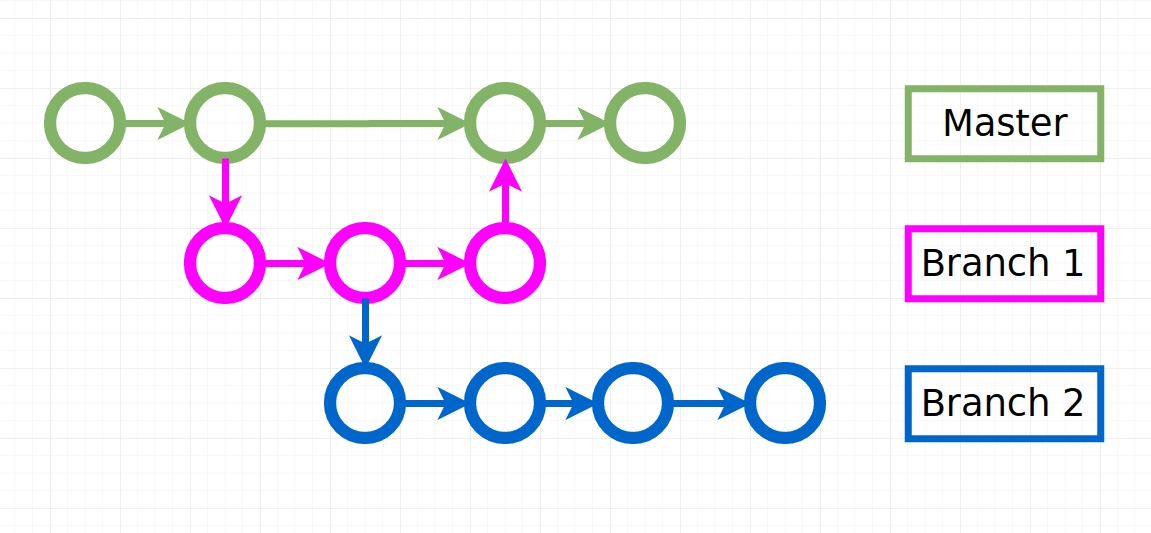
\includegraphics[scale=0.30]{images/branching.jpg}
	\caption{VCS Branching}
	\label{fig:vcs_branching}
\end{figure}

Each circle on the figure represents a commit (a group of changes). The figure also shows that branch one splits off from master, using it as its base then merged back in. While branch two uses branch one as its base, however has not yet been merged. There are different work-flows around this feature covered in more depth in section TODO:link the section.

\paragraph{VCS Systems}
So far the paper has gone on about a folder that exists, this folder goes under the name of a repository. The next part will look at where the repository is located, such that multiple people or a single person can work on the project taking advantage of VCS, and how they differ. There are two main way that this is achieved, both use a client sever architecture. 
\\\\
The first has the server contain the repository, then the developer will create a local copy of the repository according to the branch they are on. They then work on the local copy editing files, however anything else such as creating a branch, merging or checking out files is performed by the server therefore a connection is required.
\\\\
The second way is distributed and has the developer create a local repository that mimic the server one then everything can be performed locally. When a connection to the server is available they can push their changes on the the server repository. This can be seen figure \ref{fig:vcs_systems}:

\begin{figure}[H]
	\centering
	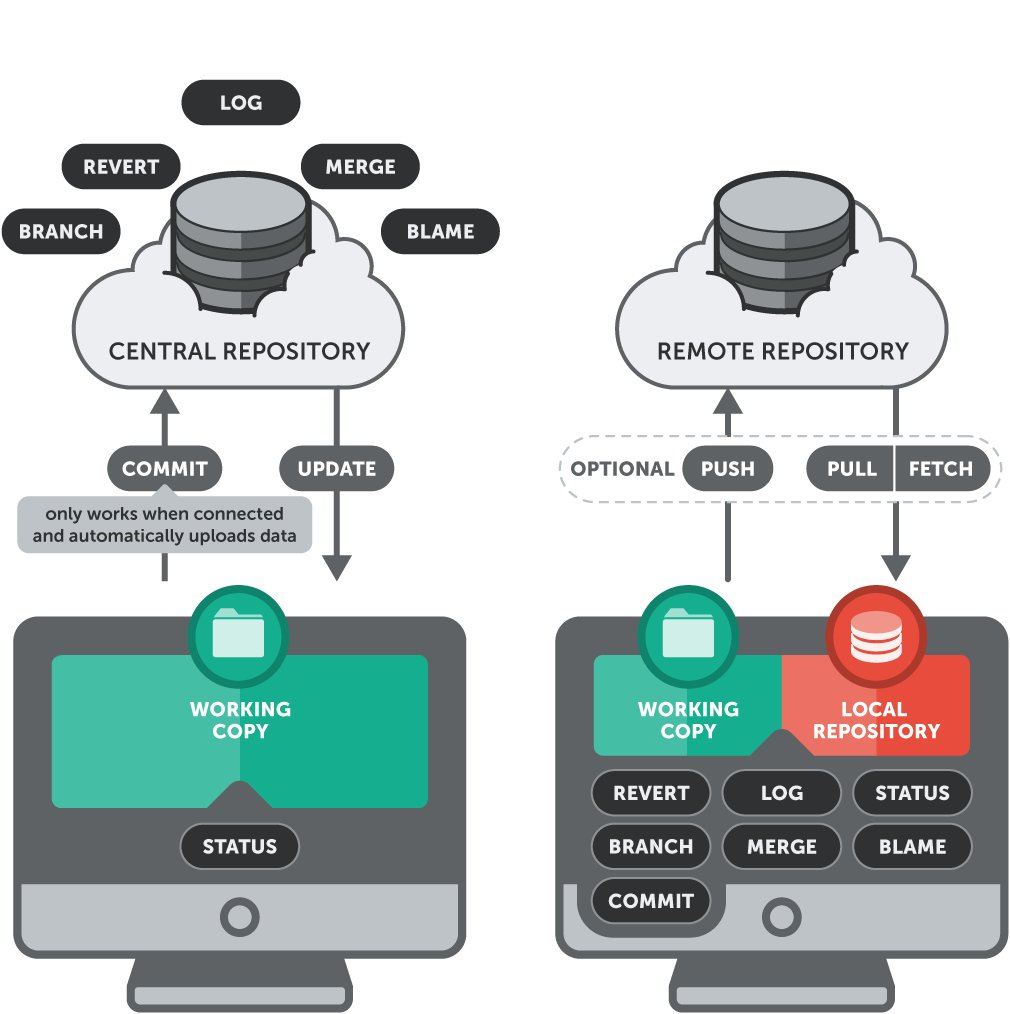
\includegraphics[scale=0.30]{images/systems.jpg}
	\caption{VCS systems modified from \cite{VCSSYSTEMS}}
	\label{fig:vcs_systems}
\end{figure}

There are a lot VCS out there, however the most popular is GIT, TFS and Subversion (\cite{vcspop}). Git follows the distributed system whereas TFS and Subversion uses the repository server system.
\\\\
There are a lot more intricate details to VCS however they will not be covered this paper.

\subsubsection{Testing}

Testing tools reefers to the frameworks used to create the mentioned unit tests and other forms of tests. In line with this paper the frameworks will be based around code testing code so it can be automated, rather then that of a manual nature.

\paragraph{Unit Testing}
Unit testing is generally the first form the tests that are run on a project, as they are fast, lightweight and give good coverage of the system. If the unit tests passed then the developer should be save in knowing that the program is in a baseline state of working order. 
\\\\
As mentioned earlier unit tests, test all public functions to make sure that each one can handle invalid and valid input correctly. The individual tests are then packed into test suites allowing the developer to run only the tests relevant to the change. In addition to helping test organisational as there are normally as many if not more lines of code in test as the project itself.
\\\\
The most popular testing framework is the xUnit family, where x is the first few letters in the language of choice, for example, JUnit for Java, CUnit for C and  CPPUnit for C++. The xUnit family  are upheld as the standard for unit testing.
\\\\
Before going any further, a quick tangent must be made into build systems. A build system takes the project and produces the final output that can then be placed where required. The build system in a basic set-up is a script that will call commands to build the project. This may involve coping files, deleting, renaming or checking that the environment has what it needs and so on.
\\\\
Therefore when building the project the build system can build the test suites as well. In a full extreme programming set up these tests will be ran automatically when the project is built. However, this does not prevent the tests from being ran without re-building, built separately or ran at all. This is covered again later in the paper. TODO: Chapter location

\paragraph{Integration and Acceptance tests}

There are other forms of testing that can be performed on a project, such as usability, regression,  and security. However, the main focus will be on integration and acceptance testing, with the rest earning a brief mention later on. TODO: Chapter location
\\\\
Unit tests tests each method individually to make sure that it is performing up to scratch, however unseen side affect may occur when these parts are put together. For example, if you have a phone case, you test that it can hold an abject of a certain size, and that it does not fall out, it will not break went dropped and more. But when you place the phone inside the case its the wrong size. This is integration testing, making sure the the each part while tested individually works as a whole.
\\\\
These test are the next step up from unit test, as in order function they will requires to simulate some of the running functionality, whereas unit tests will avoid this at all costs. For example an integration tests may require the use of a database. Whereas a unit test may fake a database just to see if the correct command is being sent.
\\\\ 
Similarly to unit tests and will be theme throughout there are frameworks that are deigned to support and run integration tests, with varying levels of sophistication.
\\\\
Following on from integration tests there are acceptance tests. Acceptance tests are performed on a fully set up system, to decide that the system is acceptable for use by the customers. This will include making sure that the system has all of the functionality available, performance and completes each task successfully. From the users perceptive.
\\\\
Acceptance tests will normally be process through the user interface (UI) that a normal user would go through. For example a web application the user would use their browser. Whereas for a command line application the testing would go trough the command line.
\\\\
For web application there are frameworks such as selenium that allow the tests to interact through a mock browser. Others will need the have a browser on the system and available to run rather than mocking. For desktop application TestFX can be used to test JavaFX application and so on.
\\\\
Overall integration and acceptance tests are designed to make sure the system can be put together and when done so will work as expected. The makes sure that when the users interact with the system that it works and does not collapse because of a glaring issue such as the phone case being the wrong size.

\subsubsection{Infrastructure}

So far the paper has looked at the where the code and other project files are stored, some of the main type of tests that are ran on a project. However, continuous deployment aims automate everything, therefore a pipeline is needed. This is where infrastructure tools step in. They act the the conveyor belt moving the project between the steps.
\\\\
At the start of the pipeline and the standard are tools such as Jenkins, Teamcity and Bamboo. Each provide a system to create steps that are then ran in order. In order to start running the steps the tools will provide several triggers.
\\\\
Triggers come in four main types, manual which will require someone to press a button to start it. Sometimes this will require typing in arguments that are needed such as the version number. 
\\\\
Time based trigger, come in two forms, when a certain time is met such as 6PM, or on a recurring frequency such as every two hours.
\\\\
The third type ties into the version control system and can trigger on a commit or every five commits or when a commit is sent to a certain branch. 
\\\\
The final type is not so much a way to start the entire process but rather a way to continuous, allow the pipeline to be triggered whenever step is completed.
\\\\
Each step in the pipeline will often be calls to other programs and then storing the logs in a central place, keeping an eye on the entire process even across machines. The support for programs such as testing and other programming language will vary from toll  to tool. Most modern tools allow sever pipeline to be running at once, it does this in the same way that  it can track the pipeline across several machines. 
\\\\
Firstly, it provides a central web server install, this is often the part that the user will interact with and set up the system. This will often require the creation of user accounts and access settings.
\\\\
Alongside the web server they will provide agents, this name will change depending on the tool. An agent is a program that will run the steps. When installed the agent will register itself to the central server allowing it to take on jobs. This allows there to be several agents on different or the same machines so several steps can be ran at once.
\\\\
Some steps however may require a specific set up for example running a Linux build of the project will not work on window. Therefore the central server will factor this into job assignment to make sure that the agent can run the job successfully. This may lead to the situation where the first three steps are ran on one agent that the next three on another due to the different requirements.